\documentclass[letterpaper,12pt]{article}
\usepackage[utf8]{inputenc}

\usepackage{rotating}
\usepackage[top=1in, bottom=1in, left=1in, right=1in]{geometry}
\usepackage{graphicx}
\usepackage[numbers,square,sort&compress]{natbib}
\usepackage{setspace}
\usepackage[cdot,mediumqspace,]{SIunits}
\usepackage{hyperref}
\usepackage{mathtools}
\usepackage{url}
\usepackage{authblk}
\usepackage{placeins}
\usepackage{float}

\onehalfspacing
\title{Measuring Astronomical Unit Using Solar Observation}
\author{Anita Bahmanyar \qquad Ayushi Singh \qquad Morten Nyborg Stostad \\Department of Astronomy and Astrophysics, University of Toronto}
\affil{\small {Written by: Anita Bahmanyar}}
\affil{\small {anita.bahmanyar@mail.utoronto.ca}}
\affil{\small {Student Number: 998909098}}
\date{April 4 2014}

\usepackage{graphicx}

\begin{document}

\maketitle

%Abstract
\begin{abstract}
\label{abstract}
In this lab our goal is to measure the Astronomical Unit (AU) which is the distance between Sun and the Earth in meters using simple geometry. The solar data was taken on March 13, 2014 as well as March 18, 2014 using the 8 inch refractor telescope located on top of the Burton Tower at University of Toronto. Using Toshiba CCD and spectrometer, we measure the rotational velocity of the sun by computing the Doppler shift between spectra of the limbs of the sun. We used two methods of covariance and Fourier Transform in order to find the wavelength shift between two edges of the sun. Using our calculated rotational velocity of the sun to be 2.044 $\pm$ 0.0480, we estimated AU to be 1.5506 $\times$ $10^{8}$ $\pm$ 3.656 $\times$ $10^6$ km which makes the true value to be 96.176 \% of the obtained value.

\section{Introduction}
\label{sec:introduction}
Astronomical distances and scales are large enough that is gets bothersome to use usual distance units such as meters and kilometers in astronomy. Therefore, astronomers have defined a new unit for distance measurements called Astronomical Unit(AU), which is defined as the distance between the Sun and the Earth. In this lab we will use simple geometry, circular motion and properties of light to measure this unit. In order to do so, we found the wavelength solution of the Charged Coupled Device(CCD) that related the pixel numbers to wavelength as explained in section 3, obtained the solar spectra along its diameter and by taking advantage of cross-correlation method as discussed in section 4, we figured out the pixel shift and from that, the Doppler Shift in the solar spectra with respect to the starting point in order to determine the radial velocity of the Sun. From this, we can compute the radius of the sun by considering the period of the Sun as known. Finally, we have all the values to compute AU using geometry as will be explained more in sections 4 and 5. The goal of this lab is to learn to find the wavelength solution for CCDs, cross-correlate data sets with each other and find the rotational velocity of the sun in order to find its radius and finally to measure AU using simple geometry as described later.


 
\section{Observation and Data Acquisition}
\label{sec:observationanddataacquisition}
\subsection{Neon and Mercury Lamps}
We used HR1 spectrometer which consists of Toshiba 1 $\times$ 3652 CCD. Size of each pixel is 8 $\mu$ $\times$ 200 $\mu$.  The wavelength range of this spectrometer is 523-573 nm. We used Neon and Mercury lamps to find the wavelength solution for this spectrometer. We set the integration times such that the pixels are not saturated. Therefore, we used 200 ms and 400 ms integration time for neon lamp and 10 ms and 50 ms integration times for the mercury lamp. We also took data of dark counts with the same exposure times for each lamp. We also took flat and dark flat data during solar observing.Table 1 shows the summery of data acquisition.


\FloatBarrier
\begin{table}[h!]
\caption{Data Summery} % title of Table
\centering % used for centering table
\begin{tabular}{| c | c | c | c | } % centered columns (4 columns)
\hline %inserts double horizontal lines
  &  Date &  Start Time [UTC] & Integration Time  \\ [0.5ex] % inserts table

%heading
\hline % inserts single horizontal line
                   
Neon &  March 5, 2014   &  22:27:03 &  199.500 \\ \hline
Neon &  March 5, 2014  & 22:38:41  &  399.000 \\ \hline
Mercury &   March 5, 2014 &  23:00:20 &  49.875 \\ \hline
Mercury &   March 5, 2014  & 23:19:44 &  9.500 \\ \hline
Sun        &  March 18, 2014  &  15:27:24      &    159.125     \\[1ex] % [1ex] adds vertical space
\hline %inserts single line
\end{tabular}
\label{table:nonlin} % is used to refer this table in the text
\end{table}
\FloatBarrier


\subsection{Solar Observing}
We went up to 16th floor of Burton Tower to use the 8-inch refractor telescope for our solar observation. We mounted another telescope cap in front of the telescope aperture in order to reduce the amount of light coming into telescope from the Sun so that the spectrum was not saturated. Then we mounted the projection screen as it can be seen in Figure 1 so that we get the Sun on the screen. Next step was to line up the shadow of the finder scope until it became circlular as in Figure 2 and then focused the the telescope to get a sharp image(We did this by looking at the sharpness of the sun spots). The next thing we considered was the temperature of the spectrometer since the spectral resolution and dispersion of the the spectrometer or in general, the wavelength solution changes with temperature and for this mean we placed the spectrometer inside a box to keep the temperature approximately as it was in the astronomy lab, where we collected Neon and Mercury data to solve for the wavelength solution. The box consisted of a resistor that heats it up. Then we connected the fibre coupler to collimate.

% images a and 2 (flat and centroids)
\begin{figure}[ht]
\centering
\begin{minipage}[b]{0.4\linewidth}
  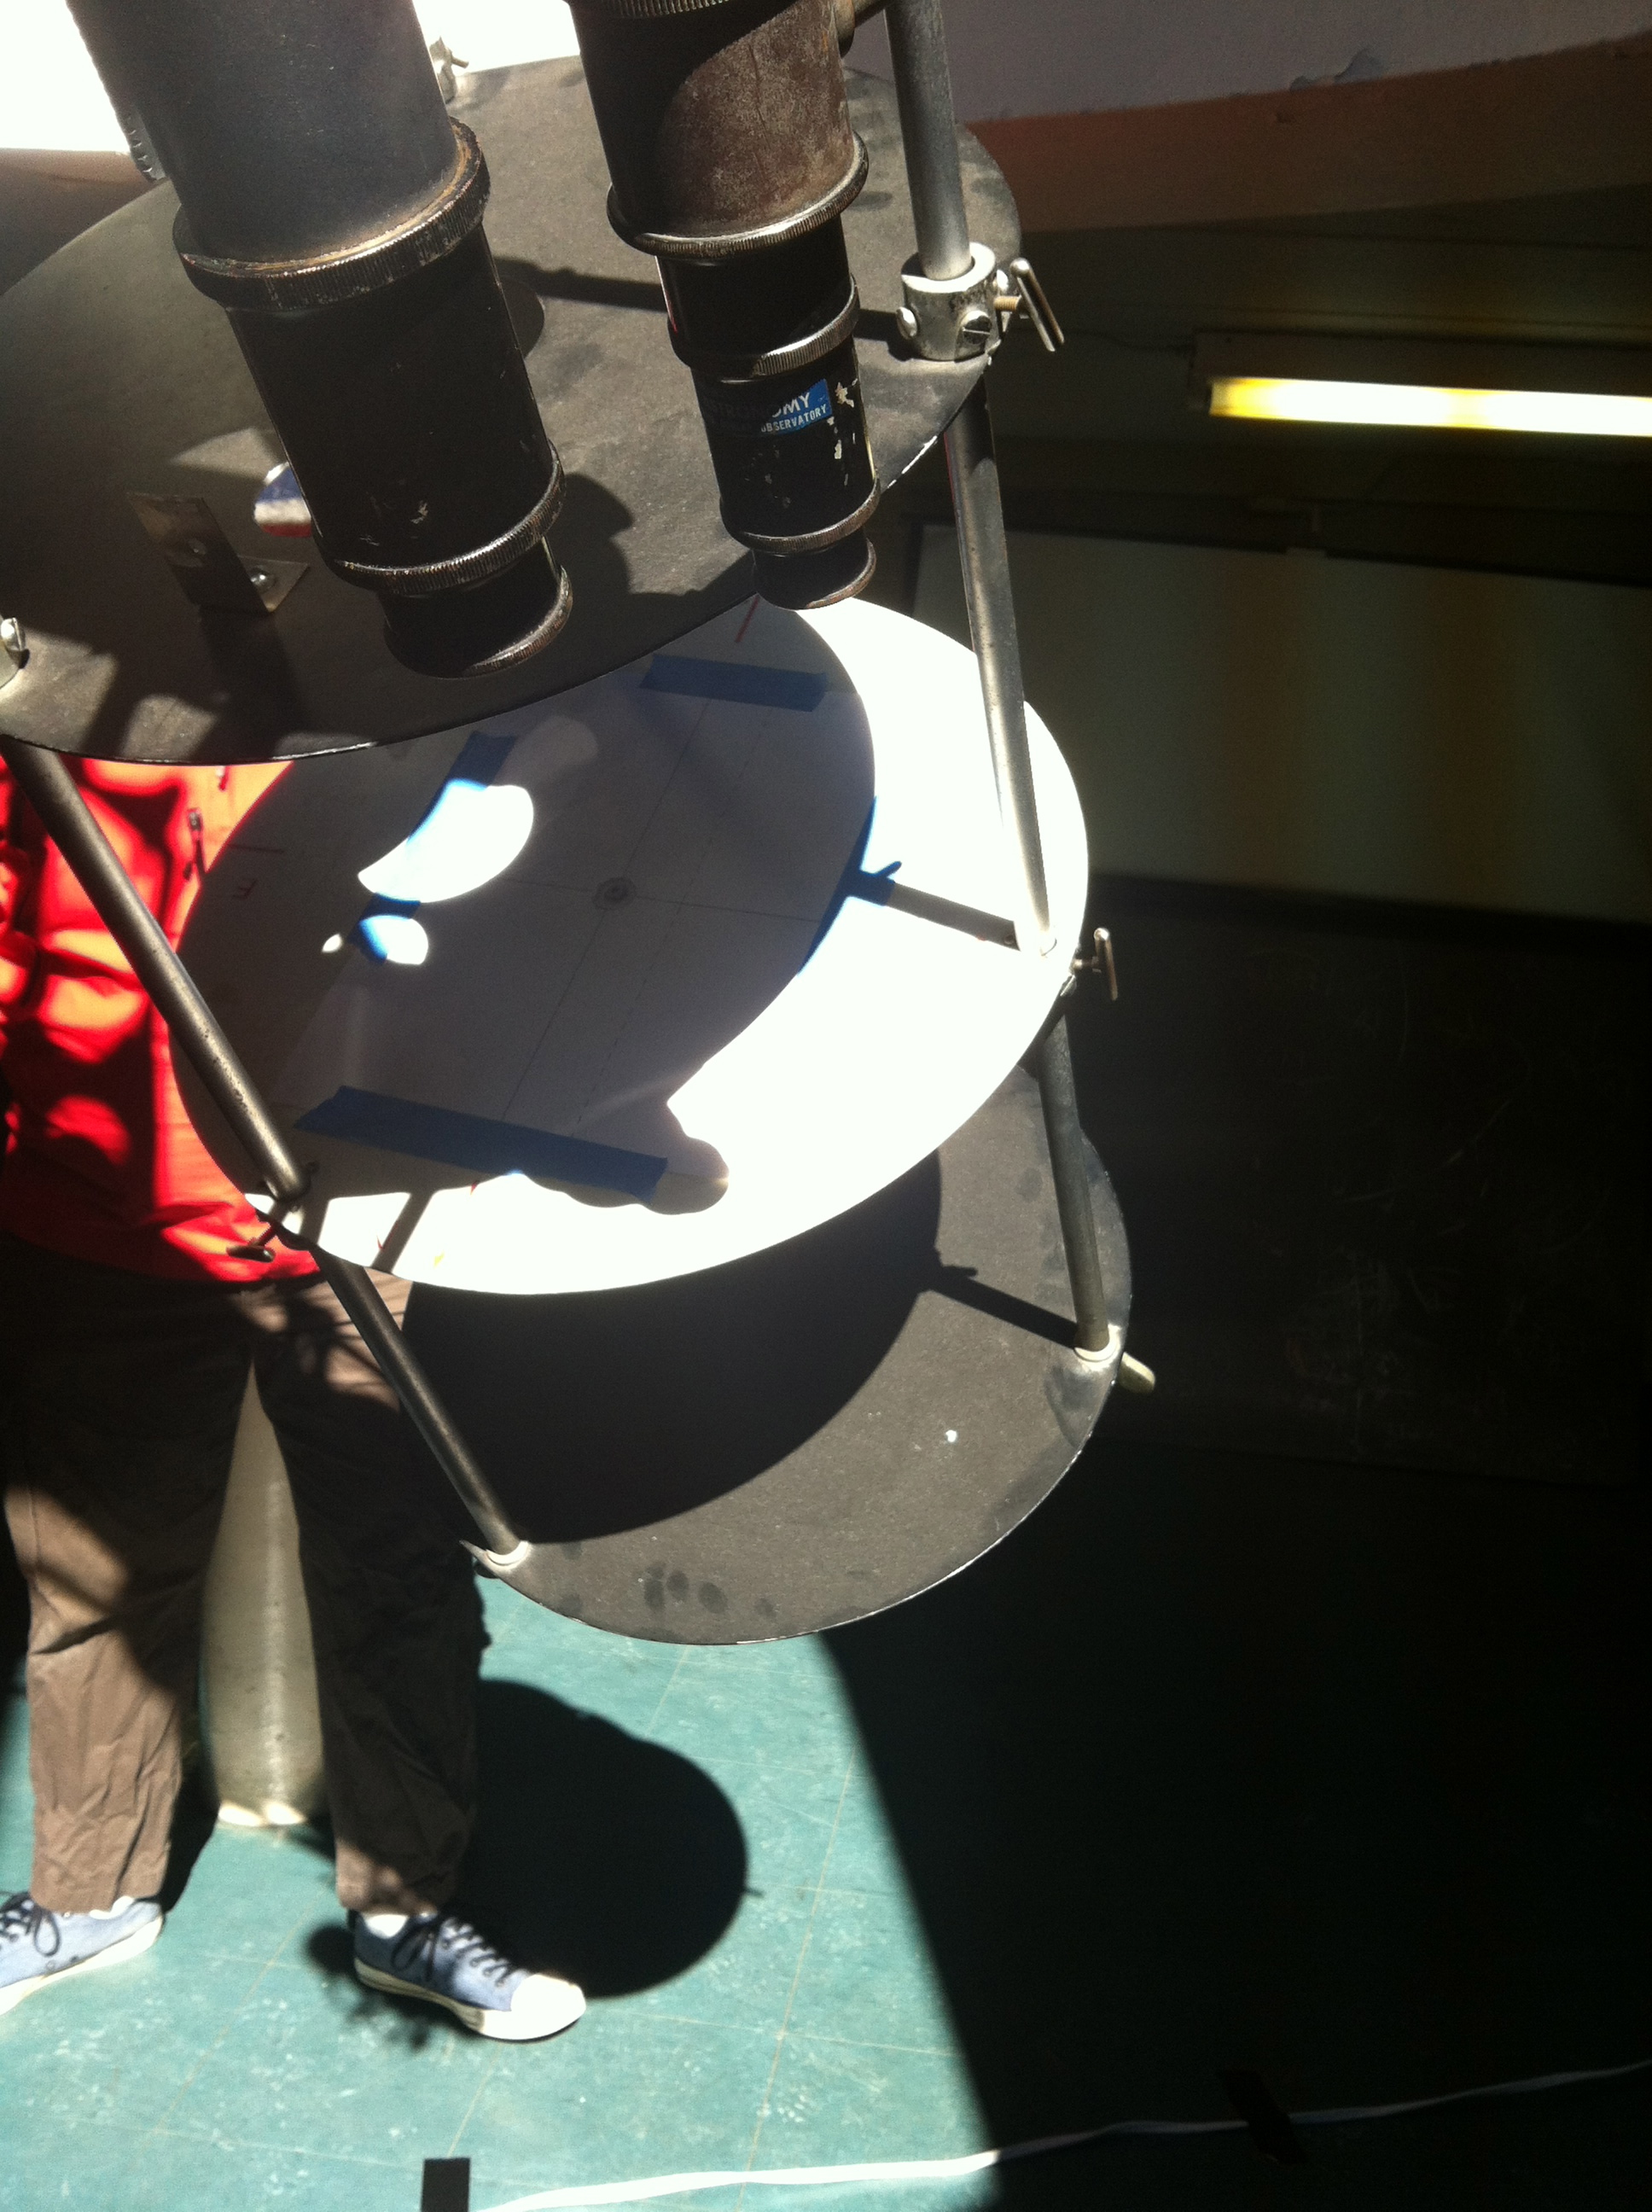
\includegraphics[scale=0.09]{projection.jpg}
  \caption{This figure shows the projection screen mounted on the telescope to get and the image of the Sun on the screen(indirect observing)}
  \label{fig:minipage1}
\end{minipage}
\quad
\begin{minipage}[b]{0.4\linewidth}
  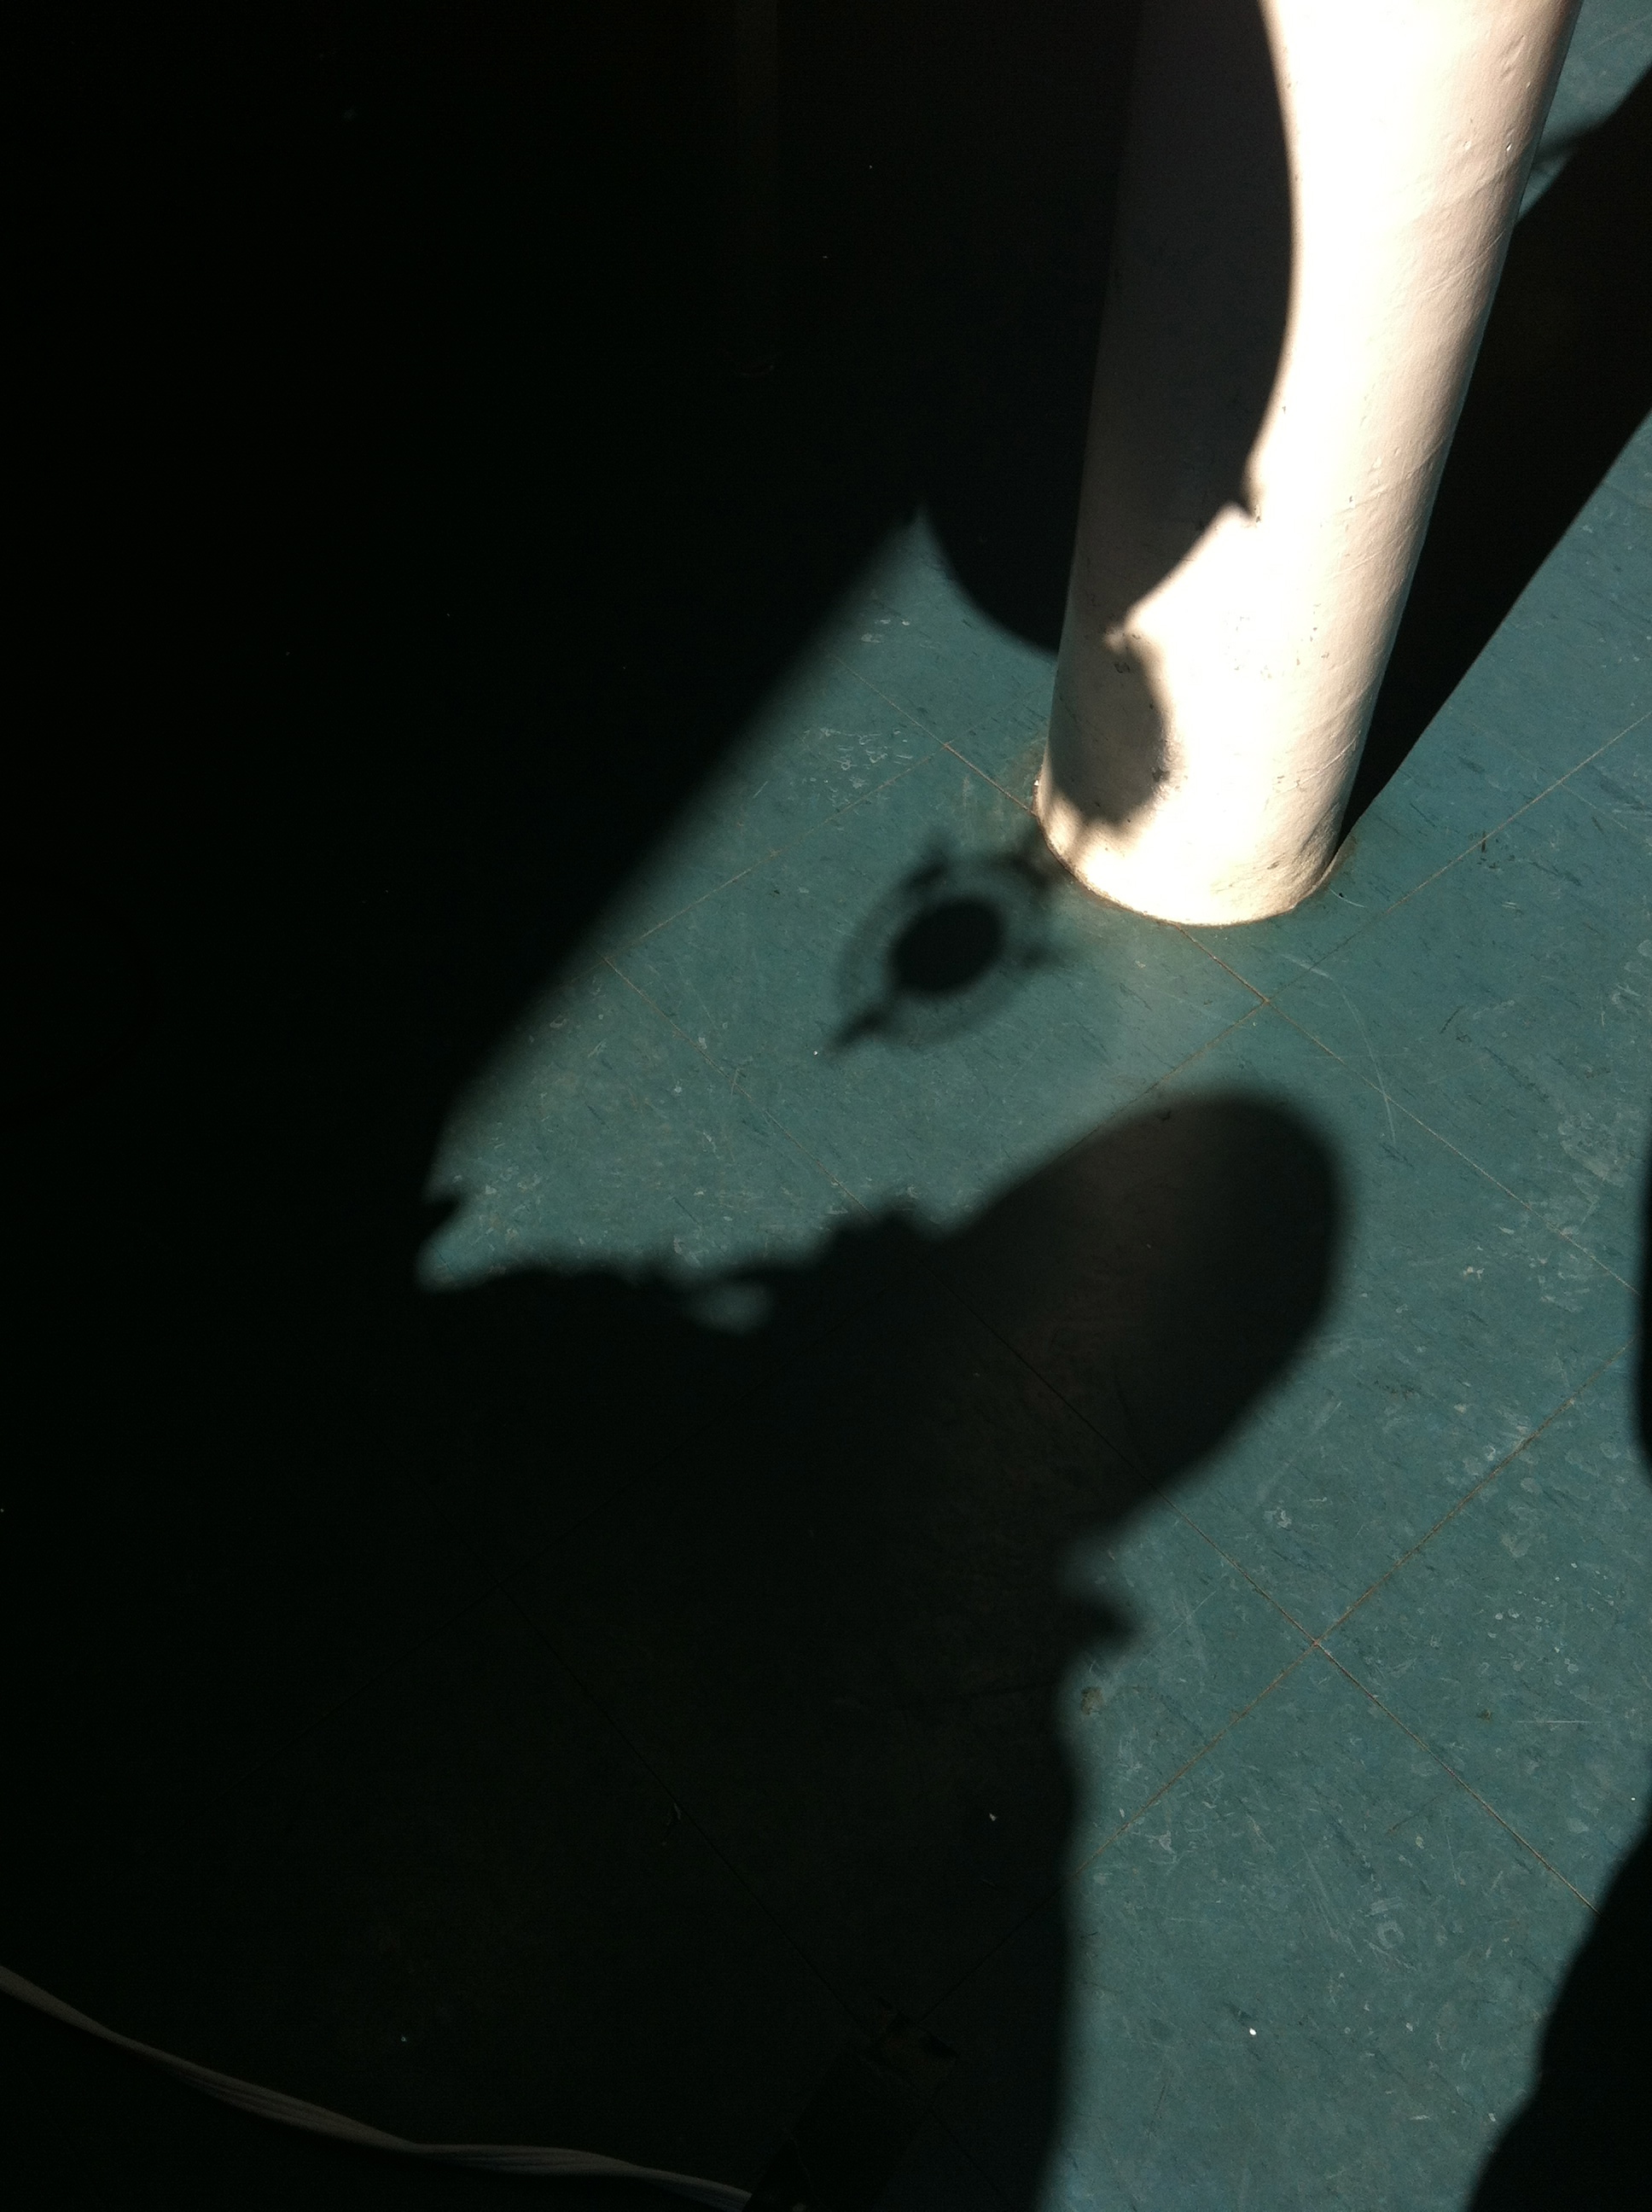
\includegraphics[scale=0.09]{finder-lineup.jpg}
  \caption{This figure shows the shadow of the finder scope as a circle which means it is lined up correctly. We also focused the telescope.}
\label{fig:minipage2}
\end{minipage}
\end{figure}




\section{Analysis}
\label{sec:analysis}
\subsection{Wavelength Solution}
We calibrated the wavelength of the spectrometer since we need to figure out how wavelength and pixel numbers are related. We used neon and mercury lamps for this purpose with the integration times tabulated in table 1. Figures 4 and 5 show the the intensity vs. pixel number of 10ms mercury and 200ms neon lamp graphs.
We then found the peaks of the graph using centroid method as discussed in Appendix section. Then we compared these peaks with a reference peak$^{[4]}$ wavelength for neon and mercury in the spectrometer wavelength range and plotted the wavelengths vs. pixel numbers in order to find the wavelength solution. We used linear least squares to fit the graph. This was done manually in Python as explained in Appendix, so it means we did not use the built-in package in Python. Fig. 3 shows the wavelength solution, which is $y= (-2.82 \times 10^{-7})x^2+ 0.015 x +523.793$, where $y$ is the wavelength and $x$ is the pixel number. 



\FloatBarrier
\begin{figure}[h!]
\centering
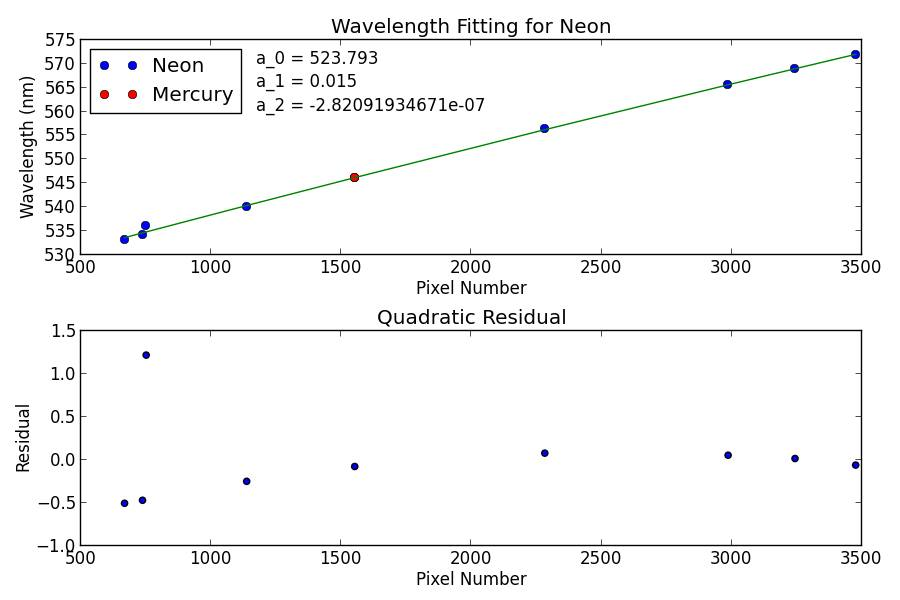
\includegraphics[scale=0.3]{wavelengh_solution2.jpg}
\caption{$Up:$ Shows the wavelengths vs. pixel numbers of neon and mercury peaks as compared with their reference spectrum. The wavelength solution is written in the graph. The lower image shows the error in the data and as it is visible it is very small and the variance is also very small that is negligible.}
\end{figure}
\FloatBarrier

\begin{figure}[ht]
\centering
\begin{minipage}[b]{0.5\linewidth}
  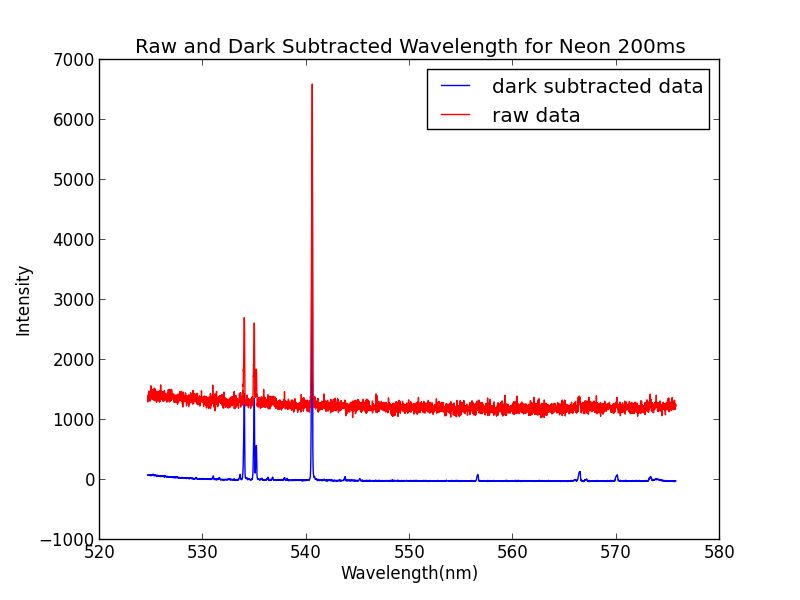
\includegraphics[scale=0.4]{wavelength_neon200ms.png}
  \caption{This figure shows the intensity vs. wavelength of neon 200ms. The raw data is very noisy unlike the mercury raw data.}
  \label{fig:minipage1}
\end{minipage}
\quad
\begin{minipage}[b]{0.4\linewidth}
  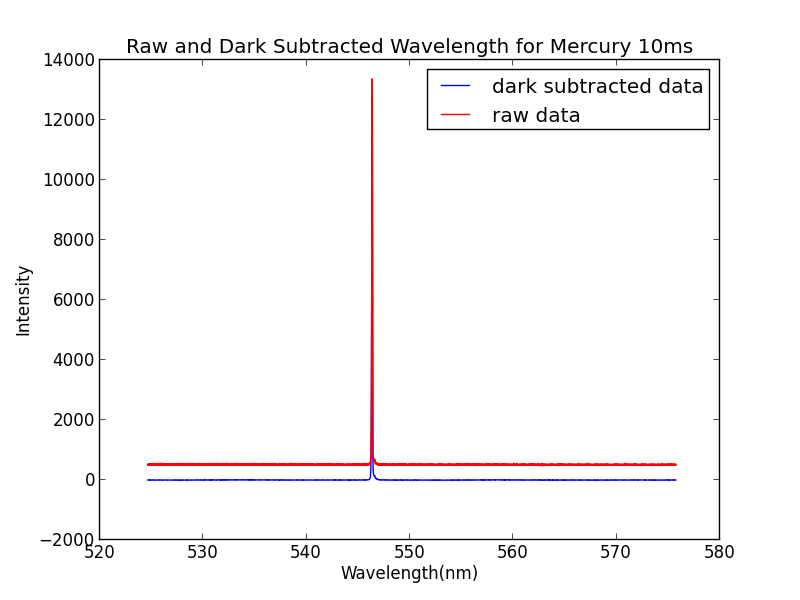
\includegraphics[scale=0.4]{wavelength_merc10ms.png}
  \caption{This figure shows the intensity vs. wavelength of mercury 10ms.}
\label{fig:minipage2}
\end{minipage}
\end{figure}

\subsection{Solar Data}
After finding the wavelength solution of the spectrometer, we should work with solar data. We collected 170ms and 200ms data sets on March 13, 2014 and three sets of data with 160ms integration time on March 18, 2014 and I used the second set of data taken on March 18, 2014. We computed the mean of each data file and plotted these mean values vs. time. The times where extracted from the file names as it will be discussed in details in Appendix. Figures 6 and 7 show this averaged value of each file vs. time, one from first observation and the other from the second observation. Then we considered the limb darkening which is given by equation 1:

\begin{equation}
I=\frac{2}{5}I_{0}(\frac{3}{5}+\sqrt{\frac{(t-t_{0})^2}{\Delta t^2}})
\end{equation}
where $I_{0}$ is the intensity of the central value of the data array, $\Delta t$ is the difference between the  time of the two limbs of the sun and $t_{0}$ is the time of the central data. Table 2 shows the values obtained from plotting averaged solar data versus time and the errors come from the fitting function. The errors from the fitting function can be obtained by computing the covariance matrix and considering the diagonal values as the errors.


% table showing the t and delta values with their errors
\FloatBarrier
\begin{table}[h!]
\caption{Limb Darkening Parameters} % title of Table
\centering % used for centering table
\begin{tabular}{| c | c | c | c | } % centered columns (4 columns)
\hline %inserts double horizontal lines
  & $I_{0} [ADU] $& $t_{center} [s]$ &  $\Delta t$ [s]\\ [0.5ex] % inserts table

%heading
\hline % inserts single horizontal line
                   
Calculated &   5087.608  &  1718.079 &  64.693 \\ \hline
Error          & 8.927 $\pm$ $10^{2}$            &   1.355e $\times$ $10^{-1}$        &       1.723 $\times$ $10^{-1}$      \\[1ex] % [1ex] adds vertical space
\hline %inserts single line
\end{tabular}
\label{table:nonlin} % is used to refer this table in the text
\end{table}
\FloatBarrier


% Limb Darkening
\begin{figure}[ht]
\centering
\begin{minipage}[b]{0.5\linewidth}
  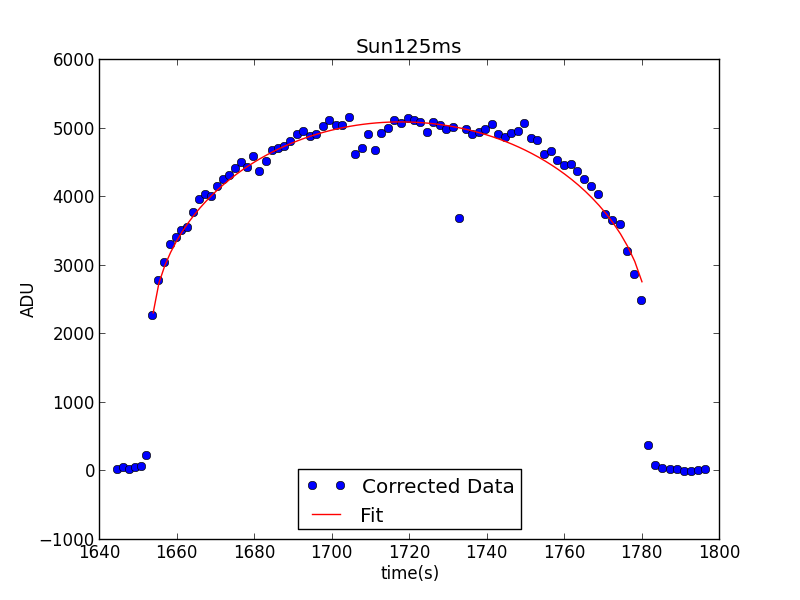
\includegraphics[scale=0.4]{11.png}
  \caption{This figure shows the intensity vs. time of sun with integration time of 125ms taken on March 18, 2014. The blue dots show the averaged spectra across the sun and the red curve shows the fit to the data. There is one dot really off from the other points which has been removed from the data for correlations that come later in the sections.}
  \label{fig:minipage1}
\end{minipage}
\quad
\begin{minipage}[b]{0.4\linewidth}
  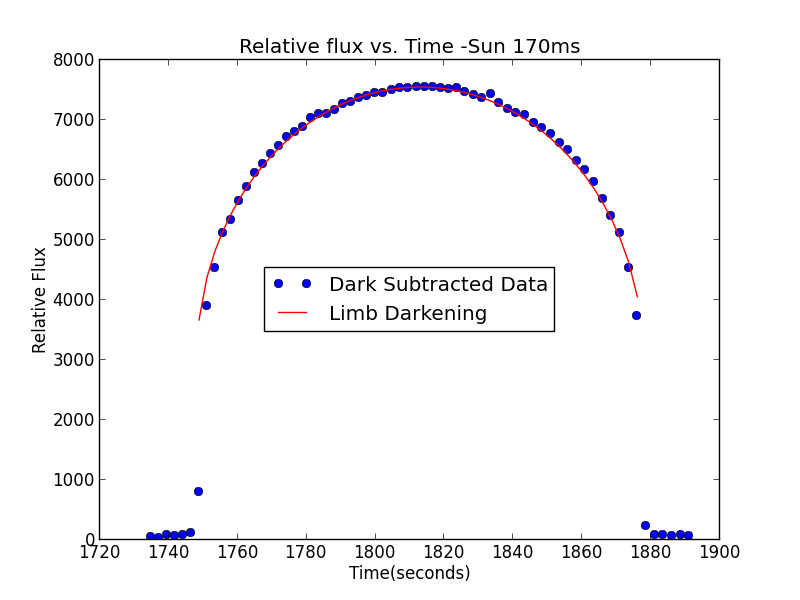
\includegraphics[scale=0.4]{sun170ms.png}
  \caption{This figure shows the intensity vs. time of sun with integration time of 170ms taken on March 13, 2014. Similar to the left picture, the blue dots show the averaged spectra and the red curve is the fit to these data points. We did not remove any of the points from the data.}
\label{fig:minipage2}
\end{minipage}
\end{figure}


\subsection{Flattening and Smoothing}
We  wanted to make the solar spectrum to look flat rather than having a blackbody shape since it is easier to see the features such as the shift and also the absorption lines. In order to do so, I tried different methods and some worked and some did not. First of all, I tried fitting a blackbody curve ($B(T)=\frac{2hc^2}{\lambda^5}\frac{1}{e^{\frac{hc}{\lambda k_{B}T}}-1}$
) to data by considering the surface temperature of the sun (5777 K), but since the spectrum is covering only a small range of the wavelength, the blackbody values did not change much and therefore division of the spectrum by the black body basically did nothing. The second method I tried was using a smoothing Python code found online called savitzky\_golay.py .This code generated a function that had a similar overall shape of our data. Fig. 8 shows the corrected solar data along with its smoothed function using this code. We should note that we should use large window sizes so that by smoothing we do not loose spectral features. Then by dividing our data by this smoother function we can get rid of the slope in the spectrum and still preserve the spectral features. However, this generated huge amount of noise at the end of the spectrum since we did not have much information on the end parts of the spectrum so the noise(uncertainty) on the end points got big. Therefore, I used a third method using gaussian functions, and it worked better than the others in that it flattened the spectrum and reduced the amount of noise at the end parts. This method convolved the data with a gaussian function using $numpy.convolve$ and then divided by the mean of these convolved data. The code explanation can be found in Appendix.

\FloatBarrier
\begin{figure}[h!]
\centering
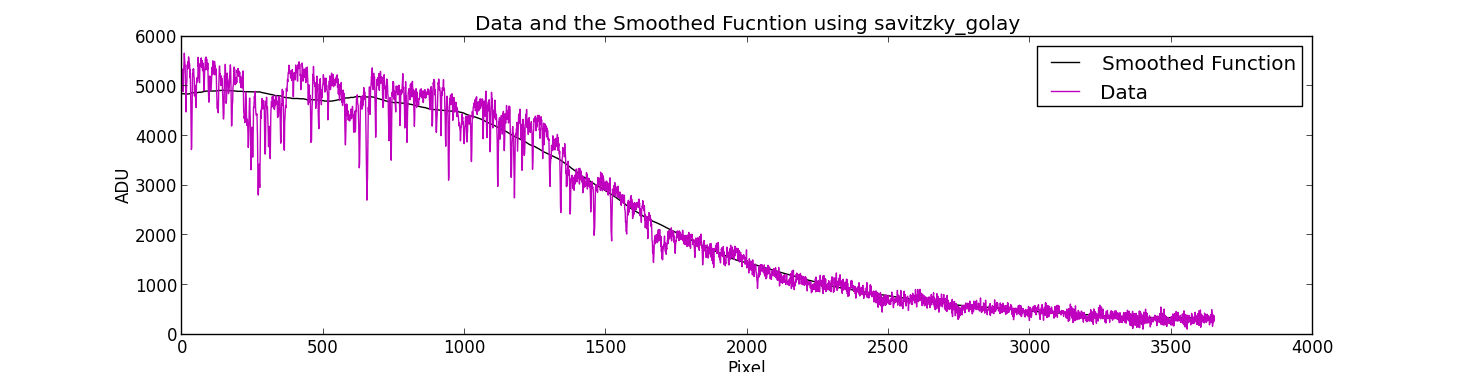
\includegraphics[scale=0.4]{savitzky.png}
\caption{This figure shows the dark subtracted and flat divided data in magenta along with the smoothed data using savitzky\_golay code. Its window size is assumed big(601) so that we do not loose the overall shape.}
\end{figure}
\FloatBarrier



% two methods of smoothing
\FloatBarrier
\begin{figure}[h!]
\centering
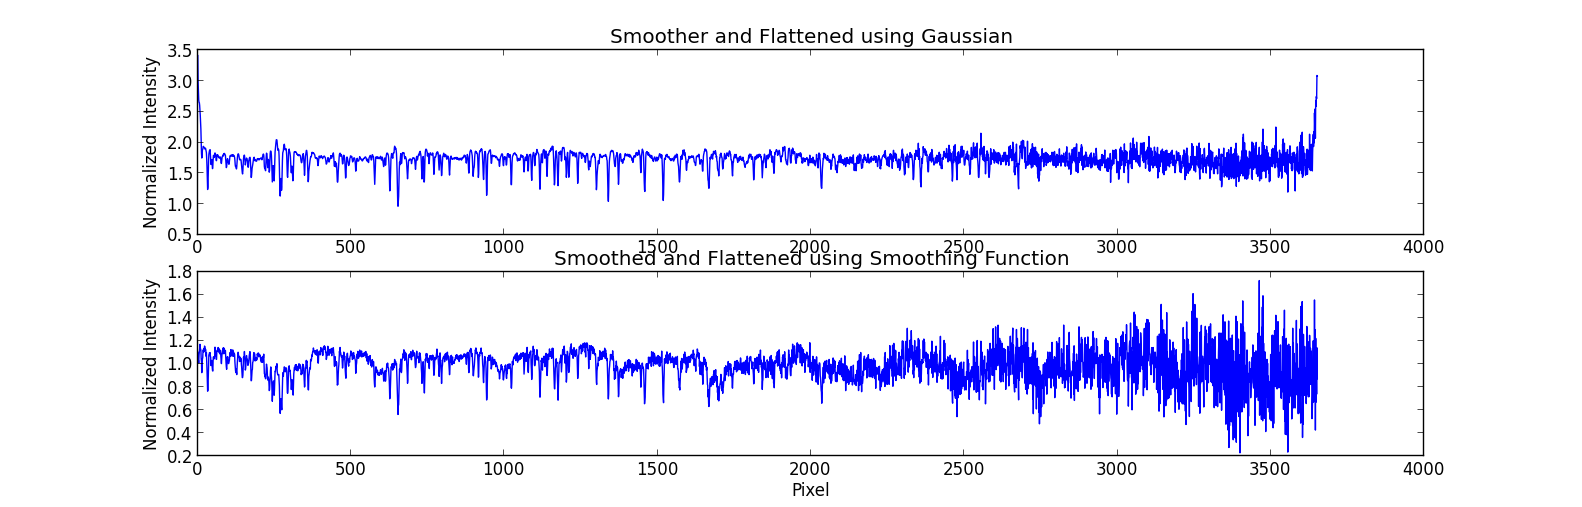
\includegraphics[scale=0.4]{subplot_flattened.png}
\caption{This figure shows flattened and smoothed spectra of the sun with two different methods. $Up:$ Smoothed and flattened using the gaussian function. $Down:$ Smoothed and flattened using savitzky golay.py code. As it is obvious using gaussian function have better results in that its end parts are less noisy and it is because in the second method we had less information about the end parts so it became more noisy at these parts.}
\end{figure}
\FloatBarrier




\subsection{Velocity Resolution of Spectrometer}
Each spectrometer has a specific velocity resolution which corresponds to its wavelength and therefore, its pixel resolving power. We used Mercury peak in the wavelength range of 523nm-573nm (since it only has one peak in this wavelength range) in order to find this velocity resolution. The method consisted of fitting a gaussian function on the peak and calculating the Full Width half Maximum(FWHM) which is given by Eq. 2:

\begin{equation}
FWHM=2\sqrt{n\ln 2}  \sigma
\end{equation}
where $\sigma$ is the standard deviation of the data. We found the $\sigma$ for the gaussian fit to be 2.816 $\pm$ 7.0532 $10^{-5}$ pixels which corresponds to FWHM of 3.315 $\pm$ 7.0532 $10^{-5}$pixels and by Eq. 3 this gives the velocity resolution of about 29.885 km/s, which is close to the 33 km/s value given in the lecture slides.$^{[3]}$ This is 90.6\% of the known value. Figure 10 shows the mercury 50ms peak and the gaussian fit on it.


% Gaussian fit image
\FloatBarrier
\begin{figure}[h!]
\centering
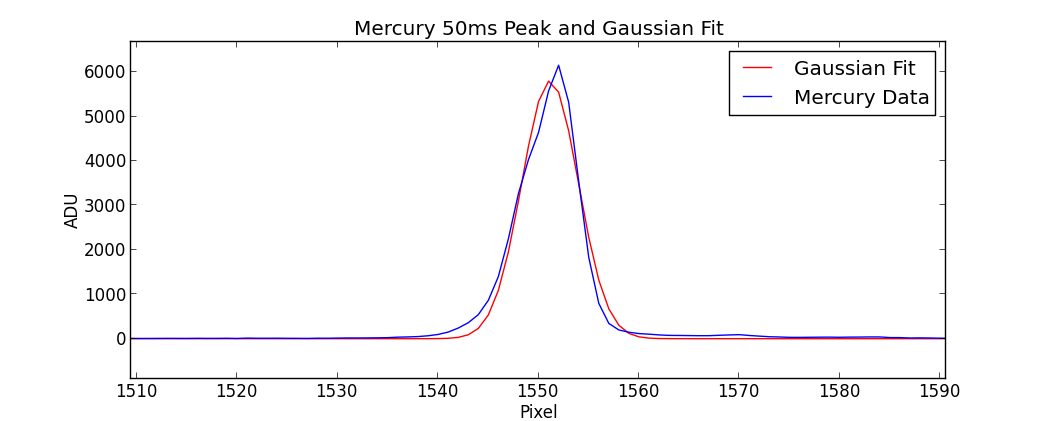
\includegraphics[scale=0.48]{velocity_resolution.png}
\caption{This figure shows the mercury 50ms peak in blue and the gaussian fit on to of it in red. We then computed the $\sigma$ of the gaussian function and used it to calculate FWHM of it in order to find the velocity resolution of the spectrometer using Doppler Shift Equation.}
\end{figure}
\FloatBarrier


\section{Determining Doppler Shift}
\label{sec:determiningdopplershift}
As we were collecting the solar data, the sun was rotating. We need to account for this rotation since it affects the wavelength of the light that we observe. As the sun rotates, one edge is turning toward us, making the light to appear blue-shifted(light has shorter wavelength) and the other edge is turning away from us, making it to appear red-shifted(light has longer wavelength). This is known as Doppler Shift and it is given by equation 3:

\begin{equation}
\frac{\Delta \lambda}{\lambda}=\frac{\Delta v}{c}=\frac{2 v_{rad}}{c}
\end{equation}

\begin{equation}
v_{rad}=\frac{c\Delta \lambda}{2\lambda}
\end{equation}
Where $\Delta v$ is the change in velocity, $\Delta \lambda$ is the change in wavelength given some reference wavelength $\lambda$ and $c$ is the speed of light in vacuum. Figure 10 shows the spectrums of the two edges of the sun. As it can be seen in the image, even the two furthest spectrums are very close to each other.


\FloatBarrier
\begin{figure}[h!]
\centering
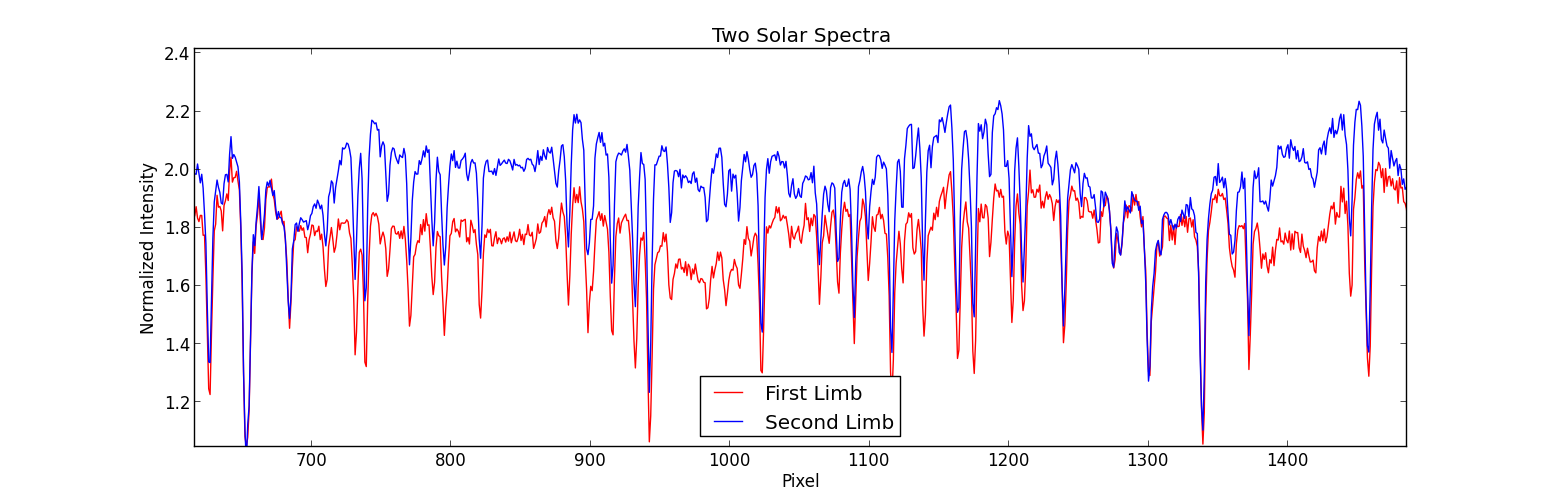
\includegraphics[scale=0.4]{limbs.png}
\caption{$Top:$ Zoomed view of two spectra of the two edges of the sun over-plotted. As it can be seen, the two spectra are very close to each other. $Bottom:$ The two spectra are zoomed so the features are better shown.}
\end{figure}
\FloatBarrier


\subsection{Cross-Correlation}
Cross-correlation is a method used in this lab in order to show how similar the different spectra are with respect to a reference spectrum of the sun. Covariance is a statistical parameter that shows how correlated two variables are. Covariance can be computed by Eq. 5:

\begin{equation}
s_{j}^2=\frac{1}{N-1}\Sigma (x_{i}-\bar x)(y_{i}-\bar y)
\end{equation}
Where N is the size of the data set, $\bar x$ and $\bar y$ are the mean values of the two data sets. In theory, the maximum value of the covariance shows where the two data sets are most similar. In order to find the shift in the pixel values of the two data sets, we considered an array from -10 to 10 and iterated it by 1 pixel each time, and computed the covariance. Then we plotted covariance vs. the array we formed. Then we should find the centroid of the cross-correlation in order to find the pixel shift. This can be computed by Eq. 6:
\begin{equation}
<j>=\frac{\Sigma_{j}jX_{j}}{\Sigma_{j}X_{j}}
\end{equation}

% Fourier Transorm
\subsection{Fourier Transform}
A Fourier Series is where any function expressed as the sum of sines and cosines. Fourier Transform also transforms a function that depends on time to a function that depends on the frequency. The way we correlated our function is given by Eq. 7:

\begin{equation}
Corr(g,h)=FFT(G(f)*H(f))
\end{equation}

% fourier transform image
\FloatBarrier
\begin{figure}[h!]
\centering
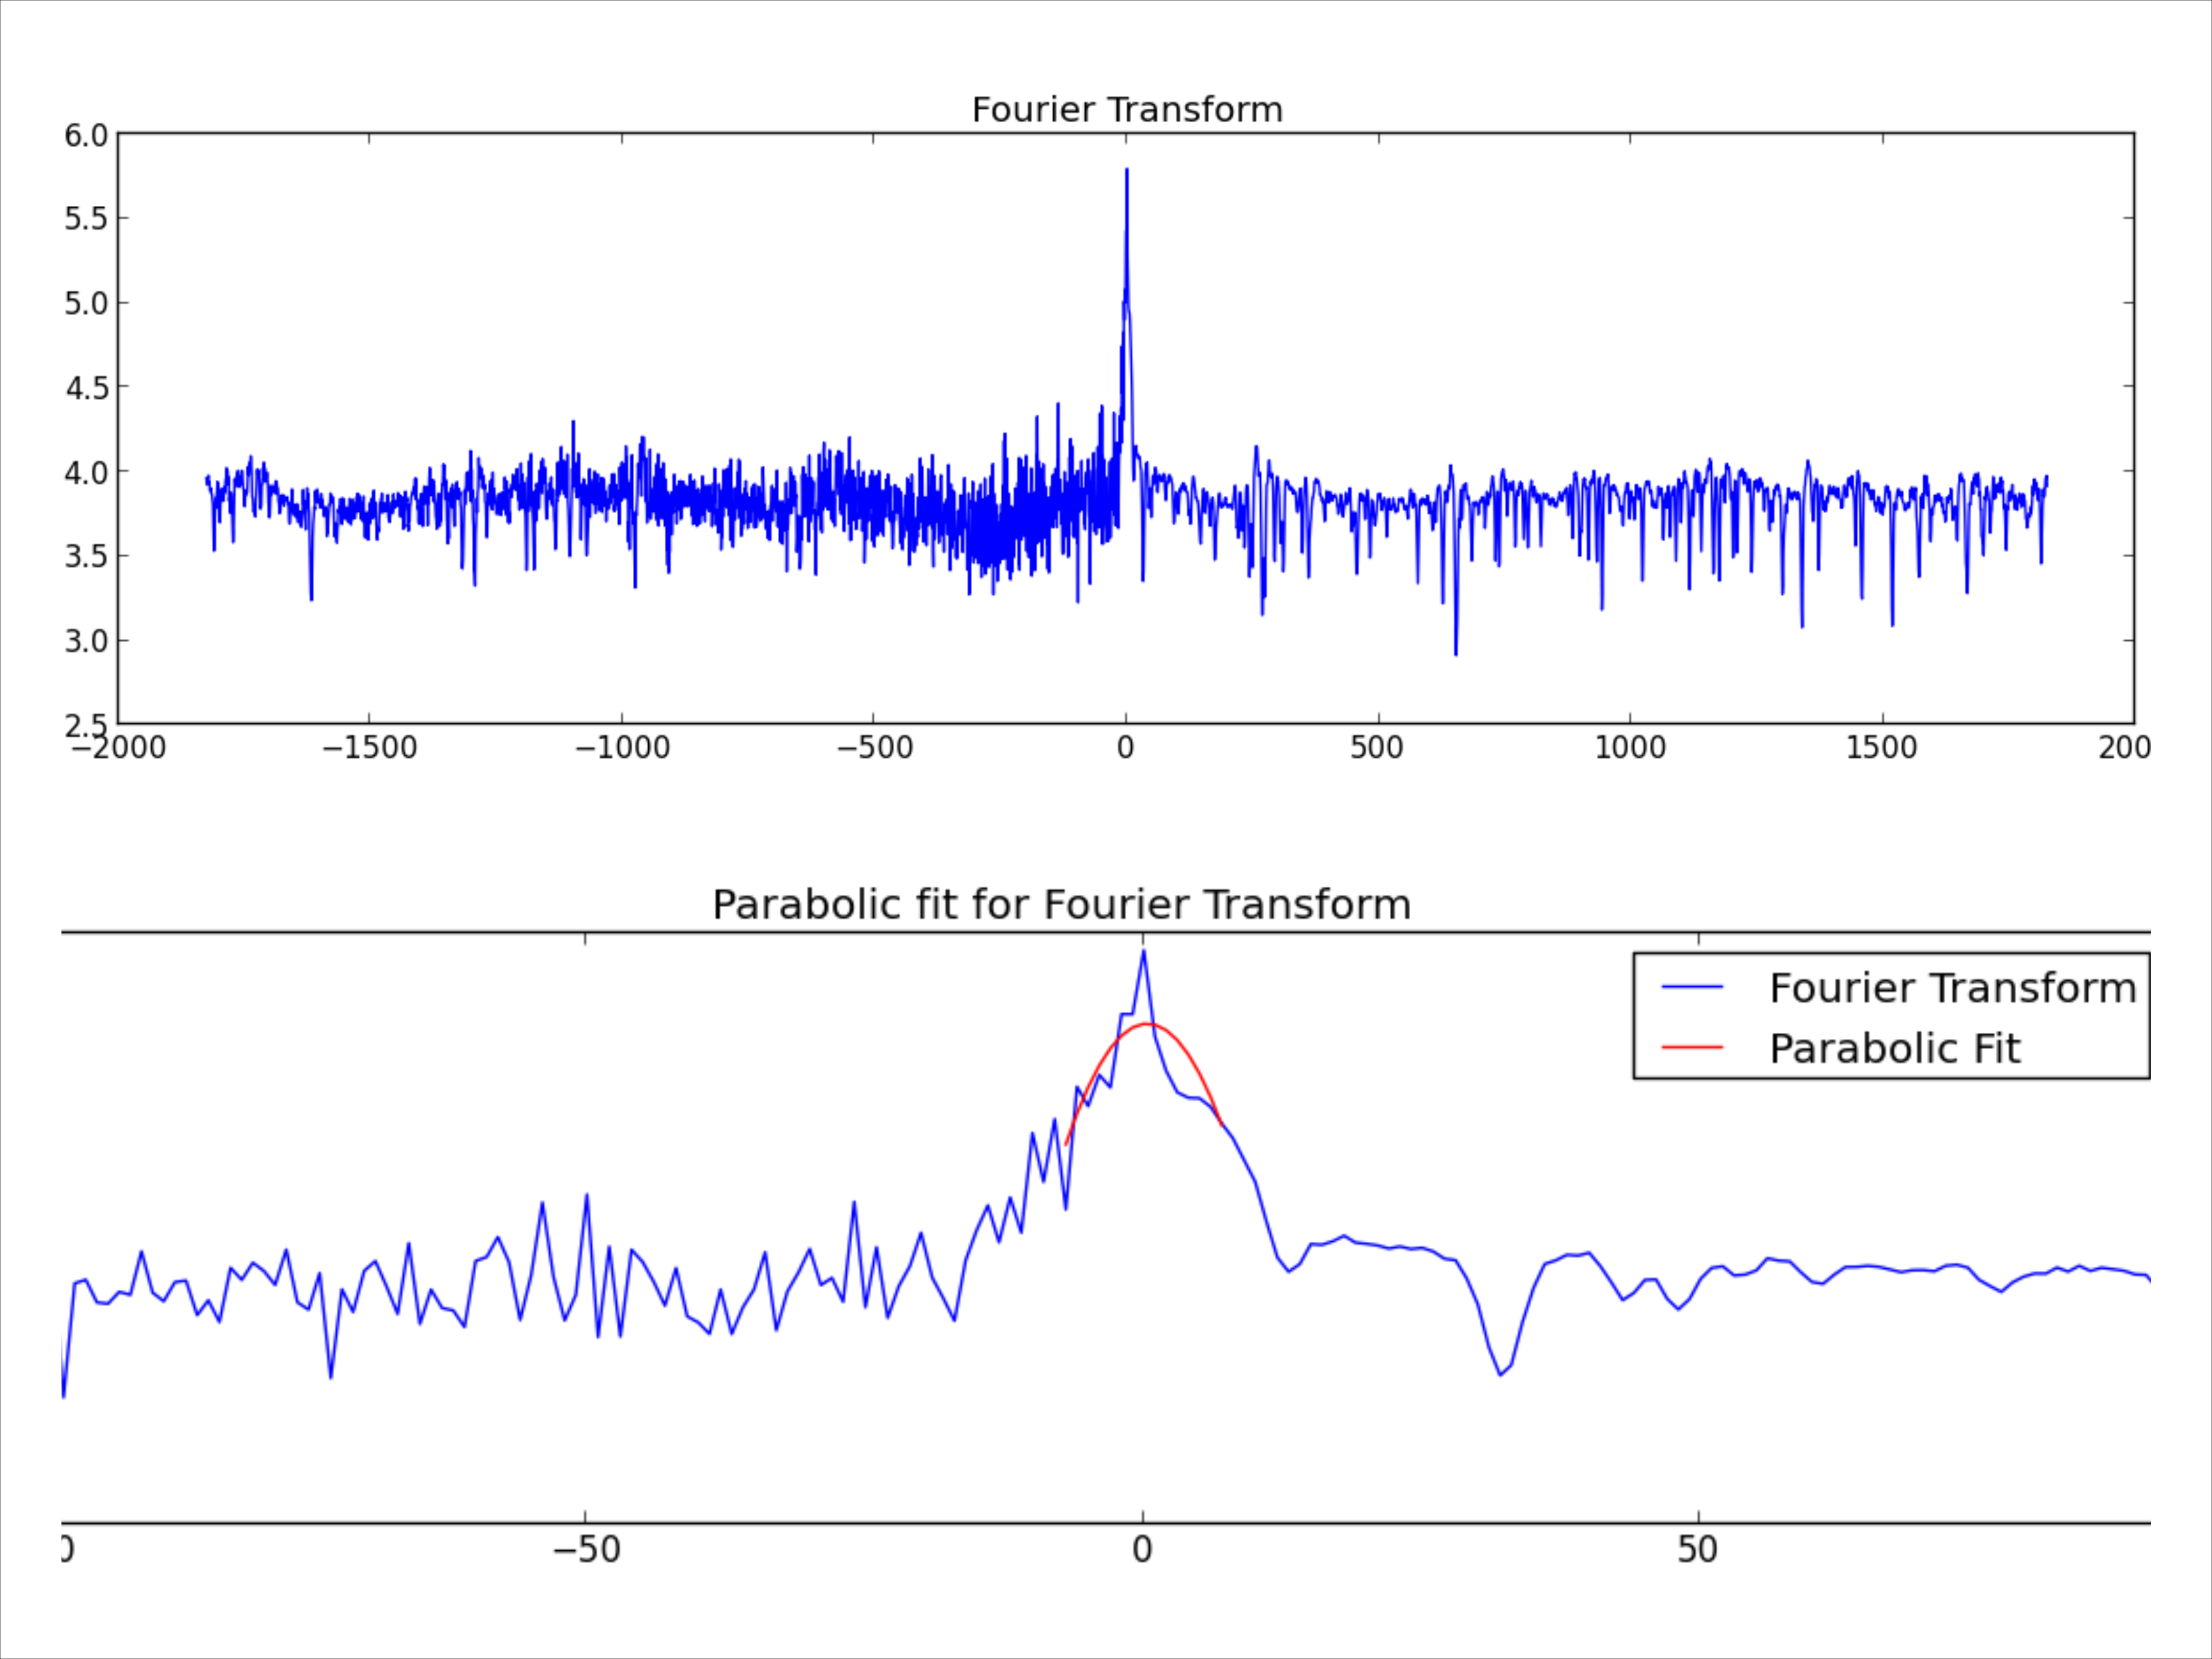
\includegraphics[scale=0.1]{fourier.png}
\caption{Fourier Transform of data. $Up:$ This is the Fourier transformed data with the peak almost at zero. The data has been rolled by amount equal to half of the data array. $Down:$ Zoomed in version of the upper image. It better shows the peak and the red curve is the parabolic fit on the peak so that we could determine the pixel shift.}
\end{figure}
\FloatBarrier


We had to roll the Fourier transformed data so that we get the peak at the center. We rolled it by half the size of the data. We then fitted a parabolic function $ax^2+bx+c$ and the values we got from are as follows: $a$=0.0131 $\pm$ 6.156 $\times$ $10^{-5}$, $b$=0.0078 $\pm$ 1.097 $\times$ $10^{-3}$ and c=5.3726 $\pm$ 4.938 $\times$ $10^{-2}$. For finding the pixel shift, we need to find the peak of the parabola which also shows the maximum point of the Fourier transformed data. We can find this point by setting derivative of parabolic equation to zero; therefore, the point would be at $x=\frac{-b}{2a}$.
Table 3 shows these values along with their errors.

% table showing parabolic fit for fourier transformed data
\FloatBarrier
\begin{table}[h!]
\caption{Parabolic Fitting to Fourier Transformed Data Parameters} % title of Table
\centering % used for centering table
\begin{tabular}{| c | c | c | c | } % centered columns (4 columns)
\hline %inserts double horizontal lines
  & $a$ & $b$ &  $c$ \\ [0.5ex] % inserts table

%heading
\hline % inserts single horizontal line
                   
Calculated &   0.0131  & 0.0078  &  5.3726 \\ \hline
Error          &   6.156 $\times$ $10^{-5}$        &       1.097 $\times$ $10^{-3}$    &     4.938 $\times$$10^{-2}$       \\[1ex] % [1ex] adds vertical space
\hline %inserts single line
\end{tabular}
\label{table:nonlin} % is used to refer this table in the text
\end{table}
\FloatBarrier


% Window function subsection
\subsection{Window Function}
In applying cross-correlation we shift the spectra relative to one another. In doing so, we beginning and the tail of the spectra would not match and line up with other spectra since our data set is finite. Since our data is discrete (we cannot integrate from $-\infty$ to $\infty$, causes the energy from the true frequency to "leak" into adjacent frequencies. Leakage is one of the most common digital signal processing errors and it cannot be eliminated completely, it can only be minimized. Therefore, we could use the window functioning method that weights the beginning and end values of the data set to zero and it also minimizes edge effects and leakage of frequencies and amplitude of the signal. In this lab we used the Hanning window function which is given by Eq. 8 below, where M is the number of points we want the window function to return:

\begin{equation}
w(n)=0.5(1-\cos (\frac{2\pi n}{M-1}))  %  0\<n\<(M-1)
\end{equation}
It is used for smoothing and it is also known as apodization which means that it "removes the foot", i.e.smoothing discontinuities at the beginning and end of the sampled signal) or tapering function. Figures 12 and 13 show different window functions and data which the Hanning window function is applied on, respectively.


% window functions
\begin{figure}[ht]
\centering
\begin{minipage}[b]{0.5\linewidth}
  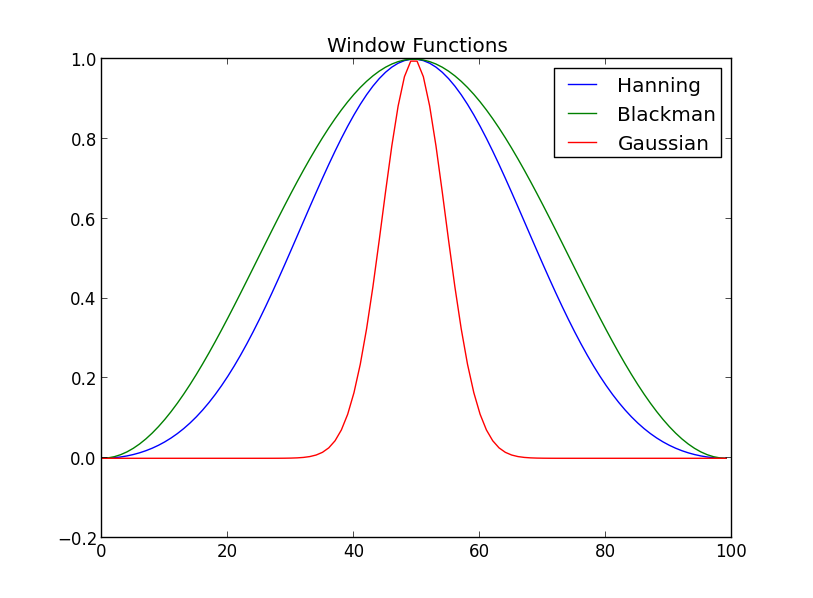
\includegraphics[scale=0.35]{window_functions.png}
  \caption{Different window functions. The blue curve shows the Hanning function that we applied on the solar data to make the end points zero.}
  \label{fig:minipage1}
\end{minipage}
\quad
\begin{minipage}[b]{0.4\linewidth}
  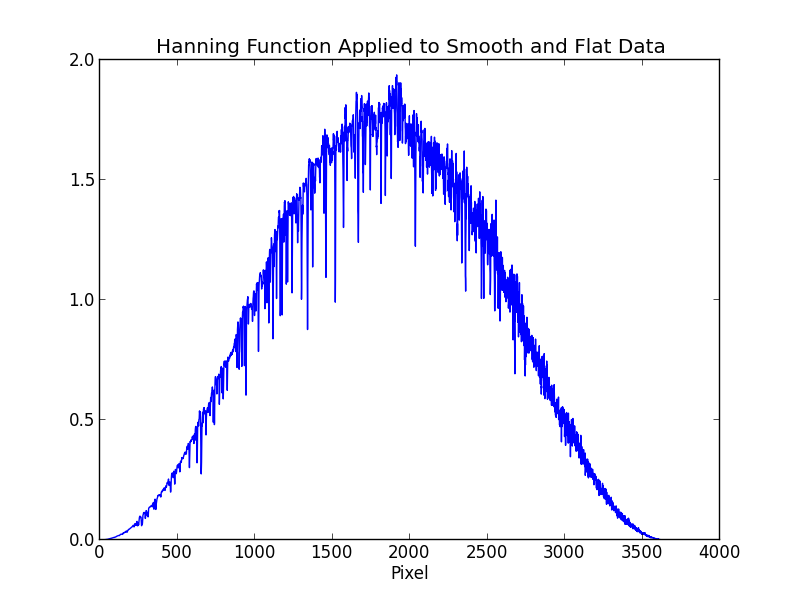
\includegraphics[scale=0.35]{hanning.png}
  \caption{Data with the Hanning function applied on. The end points are set to zero.}
\label{fig:minipage2}
\end{minipage}
\end{figure}



\section{Discussion}
\label{discussion}
Using the methods discussed in section 4, we computed the pixel shift from the two end spectra using the one that starts earlier as the reference spectrum. Then we used the wavelength solution we found for the spectrometer to convert this pixel shift into wavelength shift so that we could use Doppler Shift equation given by Eq. 3 to compute the radial velocity of the Sun. The pixel shift found is 0.408 $\pm$ 0.032 which corresponds to approximately 0.0064 $\pm$ 3.767 $\times$ $10^{-5}$ nm shift in the wavelength. The radial velocity then would be 1.839 $\pm$ 0.0432 km/s .

After applying the window function to the spectra, I recalculated the pixel shift and it was 0.411 $\pm$ 0.036, so there is a small change in the pixel shift when window function was applied.

In order to find AU, we also need to find the angular size and radius of the Sun that are given by Eq. 9 and Eq. 10, respectively. We need to find the real value of the rotational velocity of the sun in order to calculate $R_{sun}$ and this is given in Eq. 11.
%angular size equation
\begin{equation}
\frac{\Delta t}{24 h}=\frac{\theta}{360^{o}}
\end{equation}




% R sun equation
\begin{equation}
R_{sun}=\frac{v_{real} T}{2 \pi}
\end{equation}


% v real
\begin{equation}
v_{real}=\frac{v_{rad}}{\cos(\eta) \cos(\xi)}
\end{equation}

Using simple geometry, we can finally find value of 1 AU -D- which is the distance between the Sun and the Earth. Fig. 14 shows the sketch of the geometry and the math is shown by Eq. 12.

\begin{equation}
D=\frac{R_{sun}}{\tan (\theta/2)}
\end{equation}

Here, $\Delta t$ is the time between the two limbs of the sun which is twice the $\Delta t$ we used to plot the limb darkening in Eq. 1; therefore, $\Delta t$ is 126.138 $\pm$ 1.723 $\times$ $10^{-1}$. Using Eq. 9 $\theta$ has a value of 0.5256 $\pm$ 0.0007 degrees. The true angular size of the sun is approximately 0.5331 degrees as given on JPL HORIZONS$^{[1]}$ for the day of our observation, March 18, 2014; therefore, the percentage difference with the measured value and the value on JPL is  0.06 \%, which is very accurate. Tables 4 and 5 show the computed values including AU value with both methods mentioned above- covariance and Fourier transforms- along with their errors.

% simple geometry sketch
\FloatBarrier
\begin{figure}[h!]
\centering
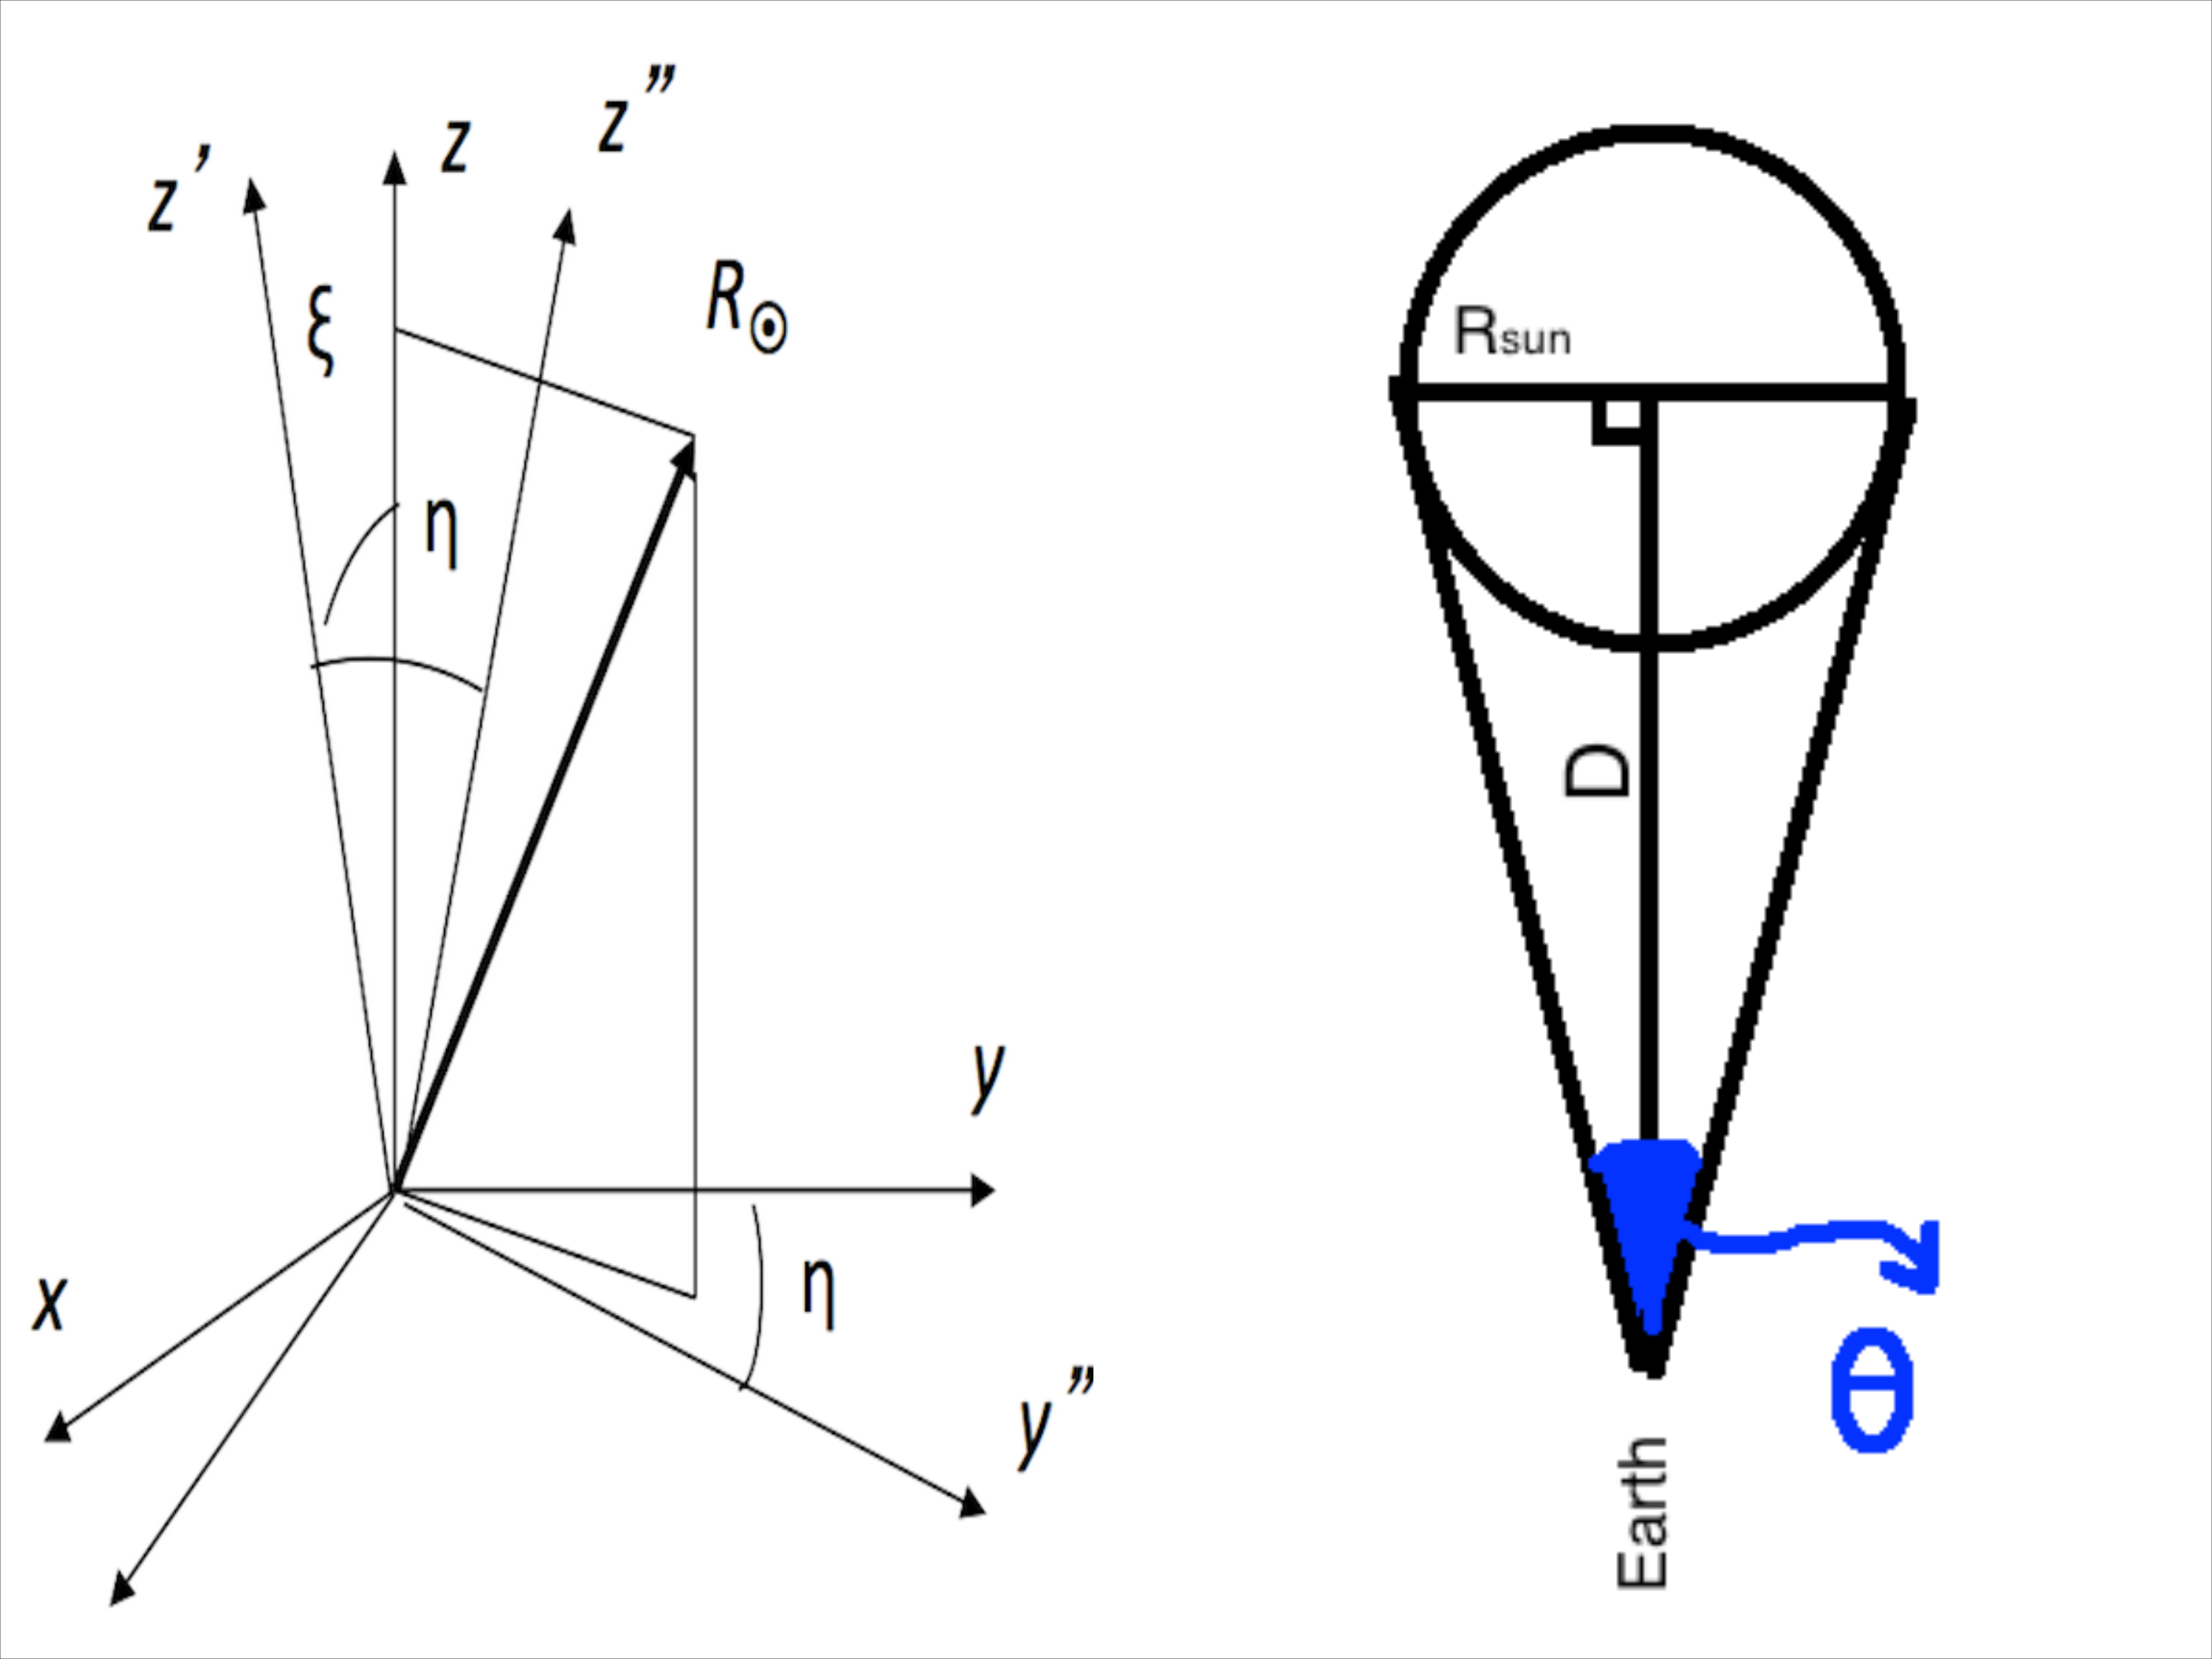
\includegraphics[scale=0.1]{transformation.png}
\caption{$Left:$Shows coordinate transformation for solar axis since it is not perpendicular to the ecliptic, meaning that the center of the sun as viewed from Earth is not b=0. Therefor, we should rotate it about y-axis by the angle $\xi$ and about x-axis by the angle $\eta$ .$Right:$This is a sketch of the simple geometry for calculating the AU using the computed values of angular size of the sun and its radius.}
\end{figure}
\FloatBarrier


% table showing all calculated values and AU
\FloatBarrier
\begin{table}[h!]
\caption{Values computed by two methods of covariance and Fourier Transforms and their errors} % title of Table
\centering % used for centering table
\begin{tabular}{| c | c | c | c | c | c |} % centered columns (4 columns)
\hline %inserts double horizontal lines
  & pixel shift &  $\Delta \lambda$ (nm) &  $\lambda$ (nm) & $v_{rad}$ (km/s) & $v_{real}$ km/s \\ [0.5ex] % inserts table

%heading
\hline % inserts single horizontal line
                   
Calculated(Covariance Method) &   0.408  & 0.0064  & 522.7807  & 1.839 &2.044 \\ \hline
Error          &     0.032         &       3.767 $\times$ $10^{-5}$       &   -   & 0.0432 &  0.0480  \\  \hline
Calculated(Fourier Method) &   0.3027  & 0.0047  &  522.7807 & 1.365 & 1.517\\ \hline
Error          &      0.057     &         3.767 $\times$  $10^{-5}$      &   -  & 0.043 &   0.048 \\[1ex]
\hline %inserts single line
\end{tabular}
\label{table:nonlin} % is used to refer this table in the text
\end{table}
\FloatBarrier




% table showing all calculated values and AU
\FloatBarrier
\begin{table}[h!]
\caption{Values computed by two methods of covariance and Fourier Transforms and their errors} % title of Table
\centering % used for centering table
\begin{tabular}{| c | c | c | c | c | c | c |} % centered columns (4 columns)
\hline %inserts double horizontal lines
  & $\theta$ (degrees)& T (days) & $\eta$(deg.) & $\xi$(deg.) & $R_{sun}$ (km) & AU (km)\\ [0.5ex] % inserts table

%heading
\hline % inserts single horizontal line
                   
Calculated(Covariance) &  0.5256   &  25.38 & 335.0652  & -7.09 & 713424.68 &155547492.76\\ \hline
Error          &   0.0007  &   -        &     -            &   -      & 16767.97      &   3655909.1 \\ \hline
Calculated(Fourier) & 0.5255   &  25.38 &   335.0652 & -7.09 & 529366.73&115417465.48\\ \hline
Error          &   0.0007  &      -    &             -    &    -     & 16767.97     & 3655909.15 \\[1ex]
\hline %inserts single line
\end{tabular}
\label{table:nonlin} % is used to refer this table in the text
\end{table}
\FloatBarrier

The value for period, observed longitude and latitude were obtained from JPL website [reference]. The pixel shift was obtained in two ways and as it is visible from the table, the covariance method had better results in terms of accuracy. The change in wavelength ($\Delta \lambda$) was also obtained from conversion of pixel shift using the wavelength solution we found. The other values were computed by the equations explained in previous sections and have small errors. In the first case that we used covariance method, the ratio of the measured AU value to the known AU value was 1.039, whereas this ratio was 0.771 using the Fourier method, so the first method was more accurate in this case.


\subsection{Error Analysis}
In order for the results to be valuable we need to show the error in the values measured as well. Here in this section I will explain how I got the errors and what are some sources of the errors that could be improved to make better results. One source of error could be the temperature of the spectrometer, since it is very temperature sensitive and the wavelength solution could change due to differences in temperatures while taking data. For this matter, people have provided a box around the spectrometer to keep it to the same temperature but it is still not completely ideal. Another source of error could be coming from the fact that we are not taking earth's rotation into account. This should not be a big deal since it is a short amount of time, but still could be taken into account for more accurate measurements. One last source of error could be fixed by finding more precise wavelength solution and it can be done by having larger range of wavelength so that we get more peaks to compare and find the wavelength solution based on.



\section{Conclusion}
\label{sec:conclusion}
I started by correcting the data by subtracting the darks and dividing by flats and found the wavelength solution of the spectrometer by comparing the pixels with wavelength as explained in section 3. Then I averaged the solar data across its surface and fitted the limb darkening function to it and got the time between two solar limbs. Then I flattened and smoothed the solar spectra using gaussian function as explained in previous sections. I choose the first limb as a reference spectrum and compared each of the other ones with it. I found the covariance for each correlation pair and plotted it.  Then we found the pixel offset by finding the centroid of these points. The other method I tried was Fourier transform and fitted a parabola to its peak to find the pixel shift and this method gave less accurate pixel offset in this case. Finally, using simple geometry discussed above, we measured value of 1 AU which is one of the standard units to measure distances in astronomy since distances between astronomical objects are large and it is hard to state them with typical distance units such as meters and kilometers.



\section{References}
\label{sec:references}
1-http://www.aseq-instruments.com/HR1.html
\\*2-http://en.wikipedia.org/wiki/Angular\_diameter
\\*3-http://www.astro.utoronto.ca/~astrolab/
\\*4-http://physics.nist.gov/PhysRefData/ASD/lines_form.html


\section{Appendix}
\label{sec:appendix}
\begin{enumerate}

\item We first discuss how we found the peaks of the spectrum of neon and mercury using centroid method. Below is the code I used to find the centroids. It goes through all of the pixels and checks the intensity value of each pixel with its neighbour pixel intensity value. If it is higher than both its left and right pixels it points as a peak.
\begin{verbatim}
for i in range(0,3652,1):
    if values[i+1]>values[i]:
        i+=1
        if values[i+1]<values[i]:
            if values[i]>70:
                Pixellist.append(i)
                centroidintensity = 0.5*(values[i]+values[i+1])
                centroidintensitylist.append(centroidintensity)
\end{verbatim}

\item Fitting wavelength vs. pixel values using linear squares.

\begin{verbatim}
ma =np.array([[np.sum(Pixels**2),np.sum(Pixels)],[np.sum(Pixels),len(Pixels)]])
mc =np.array([[np.sum(Pixels*Wavelengths)],[np.sum(Wavelengths)]])  #matrices
mai = np.linalg.inv(ma)
md = np.dot(mai,mc)
\end{verbatim}

\item  Extracting times of the solar observations from the file names.
\begin{verbatim}
times=[]
for k in range(0,66,1):
    names=np.loadtxt('sun170ms-filenames.txt',dtype='str')
    minutes=names[k][17:19]      # taking minute parts of the file name
    minutes=float(minutes)*60    # converting str to int and converting to seconds
    seconds=names[k][19:21]     # taking second parts of the file name
    seconds=float(seconds)        # converting str to int
    miliseconds=names[k][21:24] # taking mili second parts of the file name
    miliseconds=float(miliseconds)/1000 #converting str to int and to seconds
    time=minutes+seconds+miliseconds
    times.append(time)
t_center=times[5]+(times[59]-times[5])
Delta_t=(times[59]-times[5])/2
I_o=7550  #central intensity
I=I_o*((2./5)+((3./5)*(np.sqrt(1-(((times-t_center)**2)/(Delta_t**2))))))    
\end{verbatim}

\item Finding covariances("lags") using $numpy.roll$:
\begin{verbatim}
for p in range(-10,10,1):
    tester=np.roll(z[82],p)
    p_list.append(p)
    numbers=[]
    for h in range(0,3652,1):
        multiplications=(z[6][h]-mean)*(tester[h]-mean2)
        numbers.append(multiplications)
    sums=np.sum(numbers)
    sums=np.array(sums)
    covariance=1./(n-1)*sums
    covariance_list.append(covariance)
\end{verbatim}

\item Fnding the centroid of the covariance plot for each spectrum:
\begin{verbatim}
for g in range(6,82,1):
    nums=[]
    denoms=[]
    for n in p_list:
        num=(n*covariance_list[n])
        denom=(covariance_list[n])
        nums.append(num)
        denoms.append(denom)
    numerator=np.sum(nums)
    denominator=np.sum(denoms)
    cent=numerator/denominator
\end{verbatim}

\item Fourier transform method (I rolled the data by half of the data array size so that we get the peak at the center):
\begin{verbatim}
gh=(np.mean(z[5:81],axis=0))
fourier=np.fft.ifft(((np.fft.fft(gh))*(np.ma.conjugate(z[81]))))
freq=np.arange(-3652./2,3652./2,1)
rolled=np.roll(fourier,1826)
\end{verbatim}

\item Fitting parabolic function to Fourier transformed data:
\begin{verbatim}
x = freq[1819:1834]
y = rolled[1819:1834]
p0 = [0.01,0.5,0.]
def peval(x, p):  # fit function
    #mean,sig,size = p
    #return size*np.exp(-((x - mean) / sig)**2/2)/(sig*np.sqrt(2*np.pi))
    a,b,c = p
    return (-a*(x**2))+(b*x)+c
def residuals (p,y,x, peval):
    return (y) - peval(x,p)
p_final = leastsq(residuals,p0,args=(y,x, peval), full_output= True,maxfev=2000)
plt.figure()
plt.plot(x,peval(x,p_final[0]))
plt.plot(x,y)
y_final = peval(x,p_final[0])
chi2 = np.sum((y - y_final)**2)#/ ((dy)**2))
resi = (residuals(p_final[0],y,x,peval))
dof = len(y)-len(p0)
chi_re2 = chi2/dof # residual variance
cov = p_final[1] * chi_re2
\end{verbatim}

\item Smoothing using gaussian function code. It convolves the data with a gaussian function using $numpy.convolve$ and dividing the obtained values by the mean of these values.
\begin{verbatim}
def gauss_function(x, offset, a, x0, sigma):
    return offset+a*np.exp(-(x-x0)**2/(2*sigma**2))
def convolve(sun, sigma):
     sun1 = np.copy(sun)
    for i in range(len(sun1)):
        con = np.convolve(gauss_function(np.arange(-100,101), \
                                          0, 1/(sigma*np.sqrt(2*np.pi)), \
                                             0, sigma), sun1[i])
        con1 = con[100:-100]
        sun1[i] = con1
    return sun1

def smooth(sun, wvs):
    sun1 = np.copy(sun)
    sunme = np.mean(sun1[6:82], axis=0)
    divided_all = convolve(sun1[6:82], 10)
    div = np.mean(divided_all, axis=0)
    for i in range(len(sun1)):
        sun1[i] = sun1[i]/div
    np.savetxt('sunt.dat', sun1)
    return sun1
\end{verbatim}

\subsection{Error Propagation Equations}
Here are some of the equations used to calculate the errors in the values computed.
\begin{equation}
\sigma_{R_{sun}}=\sigma_{v_{real}}(\frac{T}{2 \pi})
\end{equation}

\begin{equation}
\sigma_v_{real}}=\sigma_{v_{rad}}(\frac{1}{\cos \eta \cos \xi})
\end{equation}

\begin{equation}
\sigma_{AU}=\sqrt{\sigma_{R}^2(\frac{1}{\tan(\theta/2)})^2 + \sigma_{\theta}^2(\frac{-R_{sun} \sec (\theta/2)}{\tan(\theta/2)})^2}
\end{equation}

\end{document}